\documentclass[11pt,a4paper]{amsart}

%% ─── Encoding & language ───────────────────────────────────────────
\usepackage[T1]{fontenc}
\usepackage[utf8]{inputenc}
\usepackage[english]{babel}

%% ─── Typography ────────────────────────────────────────────────────
\usepackage{microtype}
\usepackage{csquotes}

%% ─── Mathematics ───────────────────────────────────────────────────
\usepackage{amsmath, amssymb, amsthm}
\numberwithin{equation}{section}

%% ─── Page layout ───────────────────────────────────────────────────
\raggedbottom

%% ─── Lists, tables, figures & algorithms ──────────────────────────
\usepackage{enumitem}
\usepackage{booktabs}
\usepackage{graphicx}
\graphicspath{{project/figures/}}
\usepackage{placeins}
\usepackage{algorithm}
\usepackage[noend]{algpseudocode}

%% ─── Bibliography ──────────────────────────────────────────────────
\usepackage[
  backend=biber,
  style=numeric-comp,
  sorting=none,
  giveninits=true,
  doi=true,
  url=false,
  isbn=false,
  eprint=true,
  maxbibnames=99,
  maxcitenames=2
]{biblatex}
\addbibresource{seminar.bib}
\AtEveryBibitem{\clearlist{language}}
\renewcommand*{\bibfont}{\normalfont\footnotesize}  % amsart's \bibliofont
\renewcommand*{\postnotedelim}{\addcomma\addnbspace}
\AtBeginBibliography{\setlength{\emergencystretch}{1em}}  % long Serbian words

%% ─── Hyperlinks & metadata ─────────────────────────────────────────
\usepackage{hyperref}
\hypersetup{
  colorlinks=true,
  linkcolor=black,
  citecolor=blue,
  urlcolor=blue,
  pdftitle={Backpropagation for Feedforward Networks},
  pdfauthor={Elvir Muslić}
}
\usepackage{orcidlink}

%% ─── Theorem environments ─────────────────────────────────────────
\theoremstyle{plain}
\newtheorem{theorem}{Theorem}[section]
\newtheorem{proposition}[theorem]{Proposition}
\newtheorem{lemma}[theorem]{Lemma}
\newtheorem{corollary}[theorem]{Corollary}

\theoremstyle{definition}
\newtheorem{definition}[theorem]{Definition}
\newtheorem{example}[theorem]{Example}

\theoremstyle{remark}
\newtheorem{remark}[theorem]{Remark}

%% ─── Algorithms ───────────────────────────────────────────────────
\algrenewcommand\algorithmicrequire{\textbf{Input:}}
\algnewcommand{\IfThen}[2]{\State \algorithmicif\ #1\ \algorithmicthen\ #2}

%% ─── Notation shortcuts ───────────────────────────────────────────
\newcommand{\T}{\mathsf{T}}
\newcommand{\had}{\odot}
\newcommand{\norm}[1]{\lVert #1 \rVert}
\newcommand{\code}[1]{\texttt{#1}}
\hyphenation{PyTorch}

\begin{document}

%% ─── Seminar cover page ───────────────────────────────────────────
\thispagestyle{empty}
\begin{center}
  {\large University of Niš\par}
  {\large Faculty of Sciences and Mathematics\par}
  \smallskip
  Department of Computer Science\par
  Doctoral Academic Studies in Computer Science\par

  \vspace{3em}
  {\itshape Seminar paper\par}
  {\itshape Course: Artificial Neural Networks (20.IDI23)\par}

  \vspace{3.5em}
  \rule{\linewidth}{0.4pt}\par
  \vspace{1em}
  {\LARGE\bfseries Backpropagation for\\[0.35em]
    Feedforward Networks\par}
  \vspace{1em}
  \rule{\linewidth}{0.4pt}\par
\end{center}

\vspace{3.5em}
\noindent
\begin{minipage}[t]{0.49\linewidth}
  \raggedright
  \textbf{Mentor}\par
  Prof.\ Branimir Todorović
\end{minipage}\hfill
\begin{minipage}[t]{0.49\linewidth}
  \raggedleft
  \textbf{Student}\par
  Elvir Muslić\,\orcidlink{0009-0006-4042-6550}\par
  ORCID \href{https://orcid.org/0009-0006-4042-6550}{0009-0006-4042-6550}
\end{minipage}

\vfill
\begin{center}Niš, October 2026\end{center}
\newpage

%% ─── Abstract & front information ─────────────────────────────────
\begin{center}\scshape Abstract\end{center}
\noindent
Backpropagation computes the gradient of a neural network's loss with
respect to all of its weights in one pass backward through the network,
at a cost of the same order as the forward pass. This paper presents it
for feedforward networks of logistic and $\tanh$ units with half the
mean squared error as the loss: the forward pass, the three rules that
follow from the chain rule, the algorithm, and training by gradient
descent. One step is worked by hand on a network with one hidden unit.
PyTorch's automatic differentiation reproduces the hand gradient to
within ${1.4 \cdot 10^{-17}}$, and central differences agree with it to
within ${2.9 \cdot 10^{-11}}$. Trained with PyTorch by full-batch gradient
descent, a network with four hidden units learns XOR, its loss falling
from $0.1261$ to ${4.62 \cdot 10^{-4}}$, and one with sixteen classifies
all $200$ training and all $200$ test points of two interleaved half
circles correctly.

\bigskip
\setcounter{tocdepth}{1}
\tableofcontents

%% ═══════════════════════════════════════════════════════════════════
\section{Introduction}\label{sec:intro}

A feedforward network computes its output from its input through layers
of simple units, each of which forms a weighted sum of its inputs and
passes it through a fixed function. The weights are not designed but
learned from examples: training changes them until a loss, which
measures the error on the examples, is small. Gradient descent does this
by moving every weight against the derivative of the loss with respect
to it, so each of its steps needs the whole gradient, one derivative per
weight.

Backpropagation computes all these derivatives in one pass backward
through the network, from the output to the input, at a cost of the same
order as the forward pass~\cite{rumelhart1986,haykin1998}. It is the
chain rule of calculus, organized so that each intermediate result is
computed once. Rumelhart, Hinton and Williams~\cite{rumelhart1986}
showed that it lets networks with hidden layers, whose units have no
targets of their own, learn useful internal representations. Libraries
such as PyTorch~\cite{paszke2019} now carry it out by automatic
differentiation. The paper does four things.
\begin{enumerate}[leftmargin=*, nosep]
\item Section~\ref{sec:networks} describes the network, its forward pass
  and its loss.
\item Section~\ref{sec:backprop} derives the three rules of
  backpropagation from the chain rule, gives the algorithm, and works
  one step by hand.
\item Section~\ref{sec:training} explains training by gradient descent
  and checking gradients by central differences.
\item Section~\ref{sec:experiments} trains two small networks with
  PyTorch, after checking it against the step by hand.
\end{enumerate}

%% ═══════════════════════════════════════════════════════════════════
\section{Feedforward Networks}\label{sec:networks}

\subsection{The neuron}\label{sec:neuron}

A unit, or neuron, receives inputs $x_1, \dots, x_n$ and forms the
weighted sum $a = w_1 x_1 + \dots + w_n x_n + b$. Each weight $w_i$ says
how strongly, and with which sign, its input counts, and the bias $b$
shifts the sum, so that the unit can respond even when all its inputs
are zero. The output of the unit is ${h = \varphi(a)}$, where the
activation function $\varphi$ is fixed.

This paper uses two smooth, S-shaped activations: the logistic function
${\sigma(a) = 1/(1 + e^{-a})}$, with values between $0$ and $1$, and
$\tanh a$, with values between $-1$ and $1$. Their slopes follow from
their values, ${\sigma'(a) = \sigma(a)\bigl(1 - \sigma(a)\bigr)}$ and
${\tanh'(a) = 1 - \tanh^2 a}$, which the backward pass of
Section~\ref{sec:backprop} uses. This is why they must be smooth: a hard
threshold, which jumps from one value to another, has slope zero
wherever it has a slope, so the backward pass could carry nothing back
through it.

The activation must be nonlinear. Without it, every layer would be an
affine map, a weighted sum plus a constant; a chain of affine maps is
again one affine map, so a network of any depth would compute no more
than a single unit, which separates its inputs by a straight line (a
flat boundary, for more than two inputs). Section~\ref{sec:xor} shows a
problem where that is not enough.

\subsection{Layers and the forward pass}\label{sec:forward}

A layer is a group of units that receive the same inputs. A feedforward
network chains $L$ layers, each feeding the next, with no loops: the
input $x$ enters layer~$1$, and the outputs of layer~$L$ are the output
$\hat y$ of the network. Layer~$l$ has $n_l$ units; its weights form an
$n_l \times n_{l-1}$ matrix $W^{(l)}$, whose row $j$ holds the weights of
unit $j$, and its biases a vector $b^{(l)}$. With $h^{(0)} = x$, the
forward pass computes, for $l = 1, \dots, L$,
\begin{equation}\label{eq:forward}
  a^{(l)} = W^{(l)} h^{(l-1)} + b^{(l)}, \qquad
  h^{(l)} = \varphi\bigl(a^{(l)}\bigr),
\end{equation}
and returns $\hat y = h^{(L)}$; here $\varphi$ acts on each component,
and it may differ between layers. In words, each layer forms the
weighted sums of the outputs of the previous layer and passes each sum
through the activation.

Algorithm~\ref{alg:forward} states the forward pass step by step. It
keeps every $a^{(l)}$ and $h^{(l)}$, which the backward pass needs. The
layers between the input and the output are \emph{hidden}: the examples
give targets for the output only, not for them. A feedforward network of
such layers with at least one hidden layer is called a multilayer
perceptron~\cite{haykin1998}. A network with $2$ inputs, one hidden
layer of $4$ units and $1$ output unit is called a $2$-$4$-$1$ network.

\begin{algorithm}[b]
\caption{The forward pass}\label{alg:forward}
\small
\begin{algorithmic}[1]
\Require input $x$; weights $W^{(l)}$ and biases $b^{(l)}$,
  $l = 1, \dots, L$
\State $h^{(0)} \gets x$
\For{$l = 1, \dots, L$}
  \State $a^{(l)} \gets W^{(l)} h^{(l-1)} + b^{(l)}$
    \Comment{weighted sums~\eqref{eq:forward}}
  \State $h^{(l)} \gets \varphi\bigl(a^{(l)}\bigr)$
    \Comment{outputs, kept for Algorithm~\ref{alg:backprop}}
\EndFor
\State \Return $\hat y = h^{(L)}$
\end{algorithmic}
\end{algorithm}

\subsection{The loss}\label{sec:loss}

Training uses $N$ examples, pairs $(x_k, y_k)$ of an input and its
target, $k = 1, \dots, N$ (here the subscript numbers the examples, not
the components of an input). The loss scores the outputs $\hat y_k$ of
the network against the targets:
\begin{equation}\label{eq:loss}
  E = \frac{1}{N} \sum_{k=1}^{N} \tfrac12 \norm{\hat y_k - y_k}^2 .
\end{equation}
In words, $E$ is half the mean of the squared errors over the examples;
it is zero only if every output equals its target. Squaring makes errors
of either sign count, and large errors count most. The factor $1/2$
cancels the $2$ that differentiation brings down.

The loss depends on all the weights and biases through the forward
pass. Since it is a mean, its gradient is the mean of the gradients of
its terms, so Section~\ref{sec:backprop} works with one example,
$N = 1$, where $E = \tfrac12 \norm{\hat y - y}^2$.

%% ═══════════════════════════════════════════════════════════════════
\section{Backpropagation}\label{sec:backprop}

\subsection{The chain rule and the delta}\label{sec:delta}

A weight influences the loss only through a chain of intermediate
values: it changes the weighted sum of its unit, which changes the
output of the unit, which changes the weighted sums of the next layer,
and so on up to $\hat y$ and $E$. The chain rule gives the derivative
along such a chain as the product of the derivatives of its links; where
a value influences $E$ along several paths, the products of the paths
add up. Computed weight by weight, these products would repeat the same
links many times. Backpropagation computes each link once, starting from
the loss and moving backward, and it keeps the results in one quantity
per unit, the derivative of the loss with respect to the weighted sum of
the unit:
\begin{equation}\label{eq:delta}
  \delta^{(l)} = \frac{\partial E}{\partial a^{(l)}} ,
\end{equation}
a vector with one component $\delta^{(l)}_j$ for each unit $j$ of
layer~$l$. In words, $\delta^{(l)}_j$ says how much, and in which
direction, the loss changes when the weighted sum of unit $j$ changes.
It serves as the error signal of the unit and is called its
\emph{delta}; Haykin~\cite{haykin1998} uses its negative, the local
gradient.

Every weight and the bias of a unit act on $E$ only through the weighted
sum of the unit, so their gradients follow directly from its delta. The
deltas of a layer, in turn, follow from those of the next layer.

\subsection{The three rules}\label{sec:rules}

\looseness=-1 % two lines, so that Proposition 3.1 stays on one page
The two facts give three rules: one starts at the output, one sends the
deltas one layer back, and one turns each delta into gradients.

\begin{proposition}[The rules of backpropagation~{\cite{rumelhart1986}}]
\label{prop:backprop}
For one example, with the forward pass~\eqref{eq:forward} and the loss
$E = \tfrac12 \norm{\hat y - y}^2$, the deltas~\eqref{eq:delta} and the
gradients are
\begin{align}
  \delta^{(L)} &= (\hat y - y) \had \varphi'\bigl(a^{(L)}\bigr),
    \label{eq:delta-out}\\
  \delta^{(l)} &= \bigl(W^{(l+1)\T} \delta^{(l+1)}\bigr) \had
    \varphi'\bigl(a^{(l)}\bigr), \qquad l = L-1, \dots, 1,
    \label{eq:delta-rec}\\
  \frac{\partial E}{\partial W^{(l)}} &= \delta^{(l)}\, h^{(l-1)\T},
    \qquad \frac{\partial E}{\partial b^{(l)}} = \delta^{(l)},
    \qquad l = 1, \dots, L, \label{eq:grads}
\end{align}
where $\had$ multiplies two vectors component by component.
\end{proposition}

\begin{proof}
All three follow from the chain rule. Since $a^{(L)}_j$ acts on $E$ only
through $\hat y_j = \varphi\bigl(a^{(L)}_j\bigr)$, and
$\partial E / \partial \hat y_j = \hat y_j - y_j$, we
get~\eqref{eq:delta-out}. For $l < L$, $a^{(l)}_i$ acts on $E$ only
through $h^{(l)}_i$, which enters each $a^{(l+1)}_j$ with the weight
$W^{(l+1)}_{ji}$; summing over these paths gives
$\delta^{(l)}_i = \varphi'\bigl(a^{(l)}_i\bigr) \sum_j W^{(l+1)}_{ji}\,
\delta^{(l+1)}_j$, which is~\eqref{eq:delta-rec}. Last, $W^{(l)}_{ji}$
enters only $a^{(l)}_j$, with
$\partial a^{(l)}_j / \partial W^{(l)}_{ji} = h^{(l-1)}_i$, and
$b^{(l)}_j$ enters it with the derivative $1$, which
gives~\eqref{eq:grads}.
\end{proof}

In words, the output delta is the error times the slope of the output
unit; the deltas of each earlier layer are those of the next layer sent
back through the same weights, transposed, times the slopes of its
units; and the gradient of a weight is the delta of the unit it feeds
times the input it carries, that of a bias the delta itself.

\subsection{The algorithm}\label{sec:algorithm}

Algorithm~\ref{alg:backprop} puts the rules in order for one example. It
runs the forward pass, keeping every $a^{(l)}$ and $h^{(l)}$, then starts
at the output with~\eqref{eq:delta-out} and moves backward, one layer at
a time, with~\eqref{eq:grads} and~\eqref{eq:delta-rec}. The slopes come
from the kept outputs, $h^{(l)} \had (1 - h^{(l)})$ for logistic units
and $1 - h^{(l)} \had h^{(l)}$ for $\tanh$ units, so nothing is computed
twice. For $N$ examples, the gradients of the single examples are
averaged, as~\eqref{eq:loss} is a mean.

\begin{algorithm}[b]
\caption{Backpropagation for one example}\label{alg:backprop}
\small
\begin{algorithmic}[1]
\Require example $(x, y)$; weights $W^{(l)}$ and biases $b^{(l)}$,
  $l = 1, \dots, L$
\State run Algorithm~\ref{alg:forward} on $x$, keeping $a^{(l)}$ and
  $h^{(l)}$, $l = 1, \dots, L$
\State $\delta^{(L)} \gets (\hat y - y) \had \varphi'\bigl(a^{(L)}\bigr)$
  \Comment{output delta~\eqref{eq:delta-out}}
\For{$l = L, L-1, \dots, 1$}
  \State $\partial E / \partial W^{(l)} \gets \delta^{(l)} h^{(l-1)\T}$,
    \ $\partial E / \partial b^{(l)} \gets \delta^{(l)}$
    \Comment{gradients~\eqref{eq:grads}}
  \IfThen{$l > 1$}{$\delta^{(l-1)} \gets \bigl(W^{(l)\T}
    \delta^{(l)}\bigr) \had \varphi'\bigl(a^{(l-1)}\bigr)$}
    \Comment{one layer back~\eqref{eq:delta-rec}}
\EndFor
\State \Return the gradients $\partial E / \partial W^{(l)}$ and
  $\partial E / \partial b^{(l)}$, $l = 1, \dots, L$
\end{algorithmic}
\end{algorithm}

Going backward is what makes the method cheap: each delta is computed
once and serves both the weights that feed its unit and the deltas of
the layer below. The forward pass needs one multiplication per weight,
and the backward pass about two, one in~\eqref{eq:delta-rec} and one
in~\eqref{eq:grads}, which multiplies each delta by each input, so it
costs about twice as much as the forward pass, whatever the number of
weights. Central differences, the alternative of
Section~\ref{sec:training}, need two forward passes per weight.

\subsection{One step by hand}\label{sec:hand}

Take the smallest network with a hidden unit: one input $x = 1$, one
hidden and one output unit, both logistic, the weights
$W^{(1)} = W^{(2)} = 0.5$, no biases, and the target $y = 1$.
Table~\ref{tab:hand} follows the forward pass, the loss and
Algorithm~\ref{alg:backprop} line by line, in double precision. The
gradient-descent step that uses these gradients, with $\eta = 1$,
follows in Section~\ref{sec:training}.

\begin{table}[tbp]
  \centering\small
  \caption{One step by hand, with $x = 1$, $y = 1$,
    $W^{(1)} = W^{(2)} = 0.5$, no biases and logistic units: the forward
    pass, the loss and the backward pass, each row by the rule in its
    first column, to nine decimals.}
  \label{tab:hand}
  \begin{tabular}{@{}llr@{}}
    \toprule
    from & quantity & value \\
    \midrule
    forward pass~\eqref{eq:forward} & $a^{(1)} = W^{(1)} x$
      & $0.500000000$ \\
    & $h^{(1)} = \sigma\bigl(a^{(1)}\bigr)$ & $0.622459331$ \\
    & $a^{(2)} = W^{(2)} h^{(1)}$ & $0.311229666$ \\
    & $\hat y = \sigma\bigl(a^{(2)}\bigr)$ & $0.577185380$ \\
    loss~\eqref{eq:loss} & $E = \tfrac12 (\hat y - y)^2$
      & $0.089386101$ \\
    \addlinespace
    output delta~\eqref{eq:delta-out}
      & $\delta^{(2)} = (\hat y - y)\, \hat y\, (1 - \hat y)$
      & $-0.103184702$ \\
    gradient~\eqref{eq:grads}
      & $\partial E / \partial W^{(2)} = \delta^{(2)} h^{(1)}$
      & $-0.064228280$ \\
    one layer back~\eqref{eq:delta-rec}
      & $\delta^{(1)} = \delta^{(2)} W^{(2)} h^{(1)} (1 - h^{(1)})$
      & $-0.012124394$ \\
    gradient~\eqref{eq:grads}
      & $\partial E / \partial W^{(1)} = \delta^{(1)} x$
      & $-0.012124394$ \\
    \bottomrule
  \end{tabular}
\end{table}

The forward pass gives the output $\hat y = 0.577185380$, below the
target, and the loss $E = 0.089386101$. The backward pass starts at the
output: by~\eqref{eq:delta-out}, $\delta^{(2)}$ is the error
$\hat y - y$ times the slope $\hat y (1 - \hat y)$ of the output unit.
Rule~\eqref{eq:delta-rec} sends it back through $W^{(2)}$ and multiplies
it by the slope of the hidden unit, and~\eqref{eq:grads} turns each
delta into the gradient of the weight that feeds its unit. Both
gradients are negative, so increasing either weight lowers $E$ and
raises $\hat y$ toward the target.

On the way back, the delta shrinks: $\delta^{(1)}$ is $\delta^{(2)}$
times $W^{(2)} = 0.5$ and times a slope of at most $1/4$, the largest
slope of the logistic function. Over many layers, this shrinking can
slow down the learning of the first layers, a difficulty known as the
vanishing gradient.

%% ═══════════════════════════════════════════════════════════════════
\section{Training}\label{sec:training}

Training looks for weights and biases with a small loss~\eqref{eq:loss}.
Gradient descent starts from random values and repeats one step:
Algorithm~\ref{alg:backprop}, run on all $N$ examples, gives the
gradient, and the weights and biases of every layer~$l$ move against it,
\begin{equation}\label{eq:gd}
  W^{(l)} \gets W^{(l)} - \eta\, \frac{\partial E}{\partial W^{(l)}},
  \qquad
  b^{(l)} \gets b^{(l)} - \eta\, \frac{\partial E}{\partial b^{(l)}},
\end{equation}
with a step size $\eta > 0$, also called the learning rate. In words,
every weight and bias takes a step downhill, of a length proportional to
its own derivative.

So a small enough step lowers $E$, unless the gradient is zero. For a
small step, the change of $E$ is about the step times the slope of $E$
along it, and along the negative gradient that slope is as steep as it
gets: the step lowers $E$ by about $\eta$ times the sum of the squared
derivatives. Too large a step can overshoot the valley and raise $E$;
too small a step makes little progress.

On the network of Section~\ref{sec:hand}, one step with $\eta = 1$
moves the weights to $W^{(1)} = 0.512124$ and $W^{(2)} = 0.564228$, the
output rises to $\hat y = 0.587300$, and the loss falls from $0.089386$
to $0.085161$.

Gradient descent can at best reach a point where the gradient is nearly
zero, which need not have the lowest loss. For a convex loss, one that
never rises above the straight line between two of its points, a zero
gradient would mean the lowest loss; but the loss of a network with
hidden units is not convex in the weights. Exchanging two hidden units,
with their weights, leaves the loss unchanged, so its minima come in
copies, usually with a higher loss between them, which a convex loss
cannot have. Gradient descent follows the local slope only: it can stop
in a local minimum or slow down on a nearly flat stretch, and where it
ends depends on the initial weights. The experiments therefore fix the
random seed.

A backpropagation code, by hand or in a library, can be checked against
differences of the loss, which need no derivative at all. For one
parameter $\theta_j$, a weight or a bias, the central difference is
\begin{equation}\label{eq:fd}
  \frac{\partial E}{\partial \theta_j} \approx
  \frac{E(\theta_j + \epsilon) - E(\theta_j - \epsilon)}{2 \epsilon},
\end{equation}
where $E(\theta_j \pm \epsilon)$ is the loss with $\theta_j$ changed by
$\pm \epsilon$ and every other parameter fixed. In words, the slope is
measured by moving one parameter a little both ways and dividing the
change of the loss by the distance. The error of~\eqref{eq:fd} shrinks
like $\epsilon^2$, but the rounding errors of the two losses are divided
by $2 \epsilon$, so $\epsilon$ cannot be too small. A whole gradient
costs two forward passes per parameter, which makes~\eqref{eq:fd} a
check, not a way to train.

%% ═══════════════════════════════════════════════════════════════════
\section{Experiments}\label{sec:experiments}

PyTorch~\cite{paszke2019} is the method, and the step by hand of
Section~\ref{sec:hand} is the check. The notebook builds and trains the
networks with the layers, the automatic differentiation and the gradient
descent of PyTorch, which match the paper as follows.
\begin{enumerate}[leftmargin=*, nosep]
\item \code{nn.Linear} holds the weights and biases of a layer and
  computes its weighted sums, and \code{nn.Tanh} and \code{nn.Sigmoid},
  the logistic function~$\sigma$, apply the activations;
  \code{nn.Sequential} chains the layers into
  Algorithm~\ref{alg:forward}, the forward pass~\eqref{eq:forward}.
\item \mbox{\code{0.5 * ((model(X) - Y) ** 2).mean()}} is the
  loss~\eqref{eq:loss} for one output unit.
\item \code{loss.backward()} computes the gradient by automatic
  differentiation (autograd): PyTorch records the operations of the
  forward pass and applies the chain rule to them in reverse order. For
  these networks, this is Algorithm~\ref{alg:backprop} on all examples
  at once, with each delta divided by $N$, since~\eqref{eq:loss} is a
  mean.
\item \code{optimizer.step()} of \code{torch.optim.SGD} applies the
  update~\eqref{eq:gd}.
\end{enumerate}
All computations are in double precision, which the comparison of
Section~\ref{sec:check} needs. Both experiments train a network with
$\tanh$ hidden units and a logistic output unit, whose values between
$0$ and $1$ suit the targets $0$ and $1$, by full-batch gradient
descent, each step on all $N$ examples, with $\eta = 1$. They start from
the default initial weights and biases of PyTorch, which for a layer
with $n$ inputs are uniform on $[-1/\sqrt{n}, 1/\sqrt{n}]$, drawn after
\code{torch.manual\_seed(0)}. An output above $0.5$ counts as class~$1$.

\subsection{The hand step against autograd and central differences}
\label{sec:check}

Autograd reproduces the hand gradient of Table~\ref{tab:hand} to
rounding, and central differences to the accuracy that~\eqref{eq:fd}
allows. For this check, the notebook writes the loss of the network of
Section~\ref{sec:hand} as a function of its two weights and lets PyTorch
differentiate it at ${W^{(1)} = W^{(2)} = 0.5}$. Its two derivatives
differ from the hand gradient by at most ${1.4 \cdot 10^{-17}}$, a
rounding error.

The central differences~\eqref{eq:fd} with $\epsilon = 10^{-6}$ differ
from the hand gradient by ${2.2 \cdot 10^{-12}}$ for $W^{(1)}$ and
${2.9 \cdot 10^{-11}}$ for $W^{(2)}$, far above the rounding error of
automatic differentiation and far below the size of the gradients: the
rounding errors of the two losses, divided by $2 \epsilon$, limit their
accuracy.

\subsection{XOR}\label{sec:xor}

Gradient descent teaches a $2$-$4$-$1$ network the XOR function, which
no network without hidden units can represent. XOR maps the inputs
$(0, 0)$, $(0, 1)$, $(1, 0)$ and $(1, 1)$ to the targets $0$, $1$, $1$
and $0$. No straight line separates the two inputs with target $1$ from
the two with target $0$ (Section~\ref{sec:neuron}). The network has $17$
parameters and is trained on the four examples for $2000$ steps.

The loss falls from $0.1261$ to ${4.62 \cdot 10^{-4}}$
(Figure~\ref{fig:loss}), and the outputs for the four inputs are
$0.03$, $0.98$, $0.97$ and $0.04$, so all four are classified correctly.
The loss falls at every step, but not at an even pace: after $200$ steps
it is still $0.1174$, by step $500$ it is $0.0181$, and then it falls
slowly again. This is a nearly flat stretch of the kind that
Section~\ref{sec:training} describes, which this run leaves after a few
hundred steps.

\begin{figure}[tbp]
  \centering
  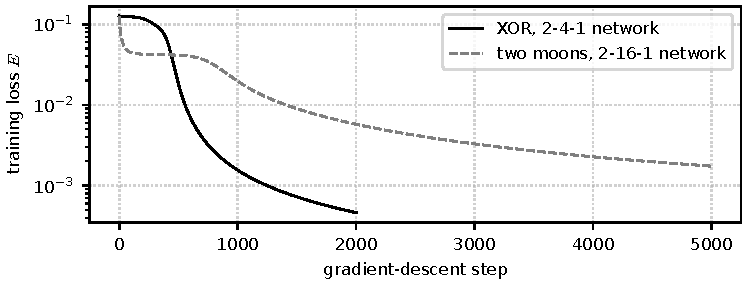
\includegraphics{training_loss.pdf}
  \caption{Training loss $E$ of~\eqref{eq:loss} at every step of
    full-batch gradient descent with $\eta = 1$: the $2$-$4$-$1$ network
    on XOR (solid) and the $2$-$16$-$1$ network on the two moons
    (dashed).}
  \label{fig:loss}
\end{figure}

\subsection{Two moons}\label{sec:moons}

A $2$-$16$-$1$ network separates two interleaved half circles, and its
boundary classifies new points from the same source correctly as well.
The data come from \code{make\_moons} of scikit-learn: the two half
circles, class~$0$ above and class~$1$ below, with Gaussian noise of
standard deviation $0.1$. No straight line separates the two arcs. The
training and the test set, $200$ points each, are drawn with the seeds
$0$ and $1$; they share the points without noise and differ only in the
noise. The network has $65$ parameters and is trained for $5000$ steps.

The loss falls from $0.1241$ to $0.0017$ (Figure~\ref{fig:loss}), again
at every step: fast to $0.0444$ within $100$ steps, then hardly, to
$0.0414$ at step $500$, and then faster again, to $0.0197$ by step
$1000$. The trained network classifies all $200$ training points and all
$200$ test points correctly. Its decision boundary, the curve on which
the output equals $0.5$, runs through the gap between the two arcs
(Figure~\ref{fig:moons}).

\begin{figure}[tbp]
  \centering
  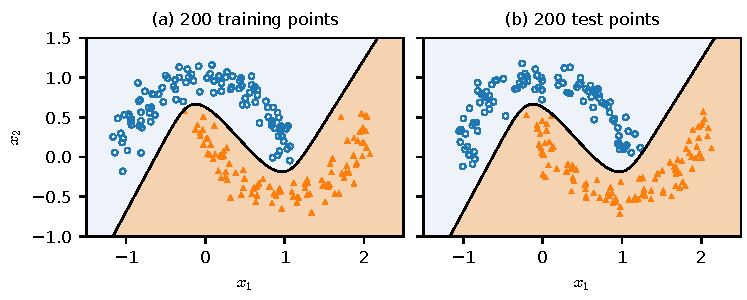
\includegraphics{moons_boundary.pdf}
  \caption{The two moons and the decision boundary of the trained
    $2$-$16$-$1$ network, the curve on which its output equals $0.5$,
    with the region of class~$1$ shaded darker: (a)~the $200$ training
    points, (b)~the $200$ test points. Open circles: class~$0$; filled
    triangles: class~$1$.}
  \label{fig:moons}
\end{figure}

%% ═══════════════════════════════════════════════════════════════════
\FloatBarrier
\section{Conclusion}\label{sec:conclusion}

\begin{enumerate}[leftmargin=*, nosep]
\item Backpropagation is the chain rule, organized backward: three rules
  (Proposition~\ref{prop:backprop}) give all the gradients in one
  backward pass, which costs about twice the forward pass.
\item On the network of Section~\ref{sec:hand}, the automatic
  differentiation of PyTorch reproduces the hand gradient to within
  ${1.4 \cdot 10^{-17}}$, and central differences to within
  ${2.9 \cdot 10^{-11}}$.
\item A $2$-$4$-$1$ network learns XOR: its loss falls from $0.1261$ to
  ${4.62 \cdot 10^{-4}}$, and all four outputs are on the right side of
  $0.5$.
\item A $2$-$16$-$1$ network classifies all $200$ training points and
  all $200$ test points of the two moons correctly.
\end{enumerate}

The findings have limits: two small problems, one run each from one
seed, plain full-batch gradient descent with one step size, and a test
set that differs from the training set only in its noise. They
illustrate the method rather than measure how well it works in general.
Faster training methods change the step, not the gradient, which
backpropagation still computes. Applied to a recurrent network unrolled
along its input sequence, the same recursion gives backpropagation
through time~\cite{werbos1990}. Recurrent networks, whose training one
of the course texts~\cite{todorovic2012} treats as the estimation of
parameters, states and structure, are outside this paper.

\section*{Code availability}

The notebook \nolinkurl{backprop_project.ipynb}, in the folder
\nolinkurl{project}, builds and trains the networks with PyTorch and
computes every number, table and figure in Sections~\ref{sec:hand},
\ref{sec:training} and~\ref{sec:experiments}. It runs on Python~3.14.7
with PyTorch~2.14.1, scikit-learn~1.9.1 and Matplotlib~3.11.2. The three
library versions, and NumPy, are pinned in
\mbox{\nolinkurl{project/requirements.txt}}; with them installed in a
virtual environment \mbox{\nolinkurl{project/.venv}} (\code{cd project},
\code{python3 -m venv .venv}, then
\code{.venv/bin/pip install -r requirements.txt}), the command
\begin{center}\scriptsize
\begin{tabular}{@{}l@{}}
  \code{.venv/bin/jupyter nbconvert -{}-to notebook -{}-execute
    -{}-inplace backprop\_project.ipynb}
\end{tabular}
\end{center}
runs it; the run reported here took a few seconds. The public repository
\url{https://github.com/innicoder/backprop-seminar} holds this paper,
its LaTeX source, the notebook with its outputs, and the figures.

\printbibliography

\end{document}
